\subsection{Datasets}
\label{sec:dataset}

Our approach to identifying relational knowledge is evaluated by using a
dataset of 40 semantic classes of almost 11,000 instances, which was
used in \cite{citeulike:1587018}.  This dataset was manually
constructed\footnote{Private communication with Marius Pasca, 2009.}
and was used to evaluate many information extraction tasks
\cite{citeulike:1587018,pacsca-vandurme:2008:ACLMain}.  Each semantic
class is an incomplete set of representative instances, and has about
272 instances in average. The smallest class is {\em search engine}
with 25 instances, and the largest class is {\em actor} with 1500
instances. Table \ref{table:class-instance} shows a snippet of the
dataset. Interestingly, we have both types of closed word semantic
class (e.g. {\em chemical element}, {\em country}), and open word
semantic class (e.g. {\em basic food}, {\em hurricane}). Moreover,
there are classes with proper nouns (e.g. {\em actor} with {\em Mel
  Gibson}, {\em Sharon Stone}), and also classes with common nouns
(e.g. {\em basic food} with {\em rice}, {\em milk}, {\em eggs}). This
fact helps evaluate the ability of systems that can deal with not only
concepts like name entities, but also common instances.

\begin{table}[h]
\small
  \centering
  \begin{tabular}{|r|l|}
    \hline
    \textbf{Semantic class (Size)} & \textbf{Examples of Instances} \\
    \hline
    \hline
    basic food (155) & rice, milk, eggs, beans, fish \\
    \hline
    chemical element (118) & lead, copper, aluminum, calcium \\
    \hline
    city (589) & San Francisco, Dubai, Chicago \\
    \hline
    disease (209) & arthritis, hypertension, influenza \\
    \hline
    actor (1500) & Kate Hudson, Mel Gibson \\
    \hline
  \end{tabular}
  \caption{A snippet of 40 semantic classes with instances. 
    The class names in the original dataset ({\em basicfood}, 
    {\em chemicalelem}) were presented in a meaningful form
    as shown in the left column.}
  \label{table:class-instance}
\end{table}

In the original dataset, the semantic class names are not often
written in a meaningful form, such as {\em chemicalelem}, {\em
  proglanguage}, and {\em worldwarbattle}. These names are not usable
for our system to find corresponding concepts in Wikipedia. In our
experiments, each semantic class name in the original dataset is
expanded to meaningful forms. For example, {\em terroristgroup} is
expanded to {{\em terrorist group}, {\em terrorrist}, {\em
    torrorism}}. The expansion is kept to be minimum. Moreover, we
also use these expansions for other systems to compare to our approach
in the experiments.

% We refer to these expansions as {\em class expansion}.

An example in our learning problem is a pair of two concepts $X$ and
$Y$ such as ({\em city}, {\em Dubai}), ({\em lead}, {\em
  aluminum}). Note that in this paper, we refer to both the name of
semantic classes and their instances as concepts. We pair the semantic
classes and instances in the original dataset to create learning examples used
in training and evaluating our approach. The examples cover all types
of relational knowledge of interest: $X \leftarrow Y$, $X \rightarrow
Y$, $X \leftrightarrow Y$, and $X \nleftrightarrow Y$. We create
learning examples with the following guidelines.

\begin{itemize}
\item $X \leftarrow Y$ examples: For each semantic class, we pair the
  name of the class with its instances. Because the order of the class
  name and the instance in a pair defines the direction of the
  relation, we make the class name and the instance as the first and
  the second concept in a pair, respectively.
\item $X \rightarrow Y$ examples: Similar to the previous guideline,
  for each semantic class, the class name and its instances are
  paired. The class name and the instance are the first and the second
  concept in a pair, respectively.
\item $X \leftrightarrow Y$ examples: For each semantic class,
  instances in the class are paired with each other. Order is not a
  matter in this case.
\item $X \nleftrightarrow Y$ examples: To make examples with two
  concepts having no relation, we pair either a class name and an
  instance of another class (and vice versa), or an instance in a
  semantic class and another instance in other classes.
\end{itemize}

Table \ref{table:examples} shows some examples in the our dataset.

\begin{table}[h]
  \centering
  \begin{tabular}{|r|l|l|}
    \hline
    {\bf Relation}          & {\bf Concept $X$} & {\bf Concept $Y$}    \\
    \hline
    \hline
    $X \leftarrow Y$        & actor             & Mel Gibson           \\
    & food              & rice                 \\
    & wine              & Champagne            \\
    \hline                               
    $X \rightarrow Y$       & Makalu            & mountain             \\
    & Monopoly          & game                 \\
    & krooni            & currency             \\
    \hline                               
    $X \leftrightarrow Y$   & Paris             & London               \\
    & copper            & oxygen                \\
    & Nile              & Volga                 \\
    \hline                               
    $X \nleftrightarrow Y$ & Roja              & C++                  \\
    & egg               & Vega                  \\
    & HotBot            & autism                \\
    \hline
  \end{tabular}
  \caption{Some examples of relations in our dataset.}
  \label{table:examples}
\end{table}

We form our learning dataset by randomly generating 20,000 examples
following the guidelines above. We divide these examples into two sets
of 8,000 and 12,000 examples for train and test sets, respectively.

For the train set of 8,000 examples, we discard any examples which
contain one or both concepts that our concept disambiguation algorithm
retrieves no relevant articles in Wikipedia. This results in a train
set of 6,959 examples. Similarly, for the test set, if we discard
examples with one or both concepts that we cannot find relevant
articles in Wikipedia, we have 10,456 out of 12,000 examples
remain. We call this test set {\em TestWiki}. The test set with all
12,000 examples is called {\em TestAll}. Table
\ref{tab:detail-dataset} presents the details of our train and test
sets with the number of examples in four relation types. In our
experiments below, we use the {\em TestWiki} test set as default,
except explicitly specified.

\begin{table}[h]
  \small
  \begin{center}
    \begin{tabular}{|l||c|c|c|c|c|}
      \hline
      Data & $X \leftarrow Y$ & $X \rightarrow Y$  & $X \leftrightarrow Y$  & $X \nleftrightarrow Y$ & Total \\
      \hline
      \hline
      Train  & 1,739 & 1,754 & 1,664 & 1,802 & 6,959\\
      TestWiki   & 2,684 & 2,654 & 2,483 & 2,635 & 10,456 \\
      TestAll & 3,045 & 3,025 & 2,965 & 2,965 & 12,000 \\
      \hline
    \end{tabular}
    \caption{Details of the training and test sets in our learning task
      with the numbers of examples in four relation types. {\em
        TestWiki} is the test set with examples having concepts in
      Wikipedia. The concepts of examples in {\em TestAll} are not
      necessarily in Wikipedia. In our experiments, we use the {\em
        TestWiki} test set as default, except explicitly specifying.}
    \label{tab:detail-dataset}
  \end{center}
\end{table}

To evaluate our system, we use a snapshot of Wikipedia in July,
2008. We first clean up articles in Wikipedia and remove articles that
are not of interest. The removed articles include articles without a
category, except the redirect pages, or articles with useless categories
such as {\em Protected redirects}. We also remove
administrative articles including {\em Wikipedia} pages, {\em
  Template} pages, {\em Image} pages, and {\em Portal}
pages. Furthermore, we do not use articles without titles. After the
pre-processing step, we have 5,503,763 articles left. These articles
will be our source to query relevant Wikipedia pages to input
concepts. We index the articles using the Apache Lucene Information
Retrieval library\footnote{http://lucene.apache.org, version
  2.3.2}. Lucene is a high-performance text search library that is
written in Java and is a widely used off-the-shelf IR system.

\subsection{Experimental Results}
\label{sec:exp-results}

In this section, we describe our experiments and evaluate the
performance of our approach in identifying relational knowledge. For
each experiment, we first present the experimental setup and then show
experimental results.

\subsubsection{Local Classifier}
We first compare the performance of our approach with other systems
that use existing resources to identify concept relation.

The first system uses a taxonomy which was derived from Wikipedia
\cite{wikitaxo07}, as the background knowledge. The taxonomy was
created by applying several lexical matching and methods based on
connectivity in the network to the category system in Wikipedia. As a
result, the taxonomy contains a large amount of subsumption, i.e. {\em
  isa}, relations \cite{wikitaxo07}.  \ignore{The taxonomy can serve
  as a source of background knowledge to identify the relational
  knowledge of interest.}  We use the taxonomy to recognize relations
between given concepts when they are in the taxonomy. Given an example
with two conceptx $X$ and $Y$, using the taxonomy, $X$ is an ancestor
of $Y$ if one of the articles about $Y$ is subsumed by an article
about $Y$. We implement this idea by looking at the {\em isa} links of
articles of $Y$ up to $K$ levels in the taxonomy.  Similarly, for the
case that $Y$ is an ancestor of $X$. If $X$ and $Y$ share a common
ancestor within $K$ levels in the taxonomy, they are considered as
siblings. We first apply our concept disambiguation algorithm on given
concepts and then mount them onto the taxonomy to infer the relations.
\ignore{To see if there is any category {\em match} with the name of
  $Y$ and its {\em class expansion}. In this case, the function {\em
    match} applying on two strings require them to be a sub-string of
  each other (including exact match) to be considered as a match. We
  can vary the value of $K$ to see the effect of going up in the
  taxonomy to the performance of relation identification.  Similarly,
  if one of the articles about $Y$ is subsumed by any article about
  $X$ in the sense that we have just described above, $X$ is
  considered as an ancestor of $Y$. For the case where one of the
  articles about $X$ and one of the articles about $Y$ have a least
  common subsumption, we conclude that they are holding a sibling
  relation. This idea is implemented by checking if there is any exact
  match between categories of the articles of $X$ and categories of
  the articles of $Y$ up to $K$ levels in the taxonomy. If none of the
  decision above is made, the two concepts are considered as holding
  no relation. Because the taxonomy derived from \cite{wikitaxo07}
  contains only the titles of articles in Wikipedia, we first apply
  our concept disambiguation algorithm on an input pair to get two
  lists of articles relevant to two concepts in the pair. From these
  lists of articles, we mount two concepts onto the taxonomy by
  looking for the titles of articles in the taxonomy.}  The taxonomy
used in this experiment is in the latest version of March,
2008\footnote{Private communication with Michael Strube and Simone
  Paolo Ponzetto, 2009.}. We refer to this system as {\em Strube 07}
in our experiment.

The second system that we compare to in this experiment uses the {\em
  extended WordNet} \cite{ilprints665,Snow2006} as the background
knowledge. The authors of the extended WordNet \cite{ilprints665}
first identified lexico-syntactic patterns indicative of hypernymy
from corpora. These patterns were used to extract candidate noun pairs
that may hold the hypernym relation. A trained classifier is applied
on these noun pairs to recognize the pairs holding hypernym relation.
\ignore{For each candidate noun pair, the authors applied a trained
  hypernym-only classifier on its feature count vector, which had
  69,592 dimensions of dependency pathes connecting two nouns of
  interest, to identify if the candidate pair holds a hypernym
  relation. Furthermore, the authors of the extended WordNet expanded
  the learning model of hypernym classification by combining it with a
  coordinate term (sibling) classification to have a hybrid
  hypernym-coordinate classification. In their later work
  \cite{Snow2006}, the authors of the extended WordNet incorporate
  evidence from multiple classifiers over heterogeneous relationships
  to optimize the entire structure of the taxonomy (WordNet 2.1, in
  this case), using knowledge of a word's coordinate terms to help in
  determining its hypernyms, and vice versa.}  Starting from
WordNet-2.1 \cite{Fellbaum98}, the latest version of the extended
WordNet has augmented 400,000 synsets. Words that are added into the
extended WordNet can be common nouns or proper nouns. The extended
WordNet can serve as the very good background knowledge to identify
relational knowledge of interest by looking for input concepts in the
extended WordNet taxonomy for all possible senses of the
concepts. Given a pair of two concepts ($X$, $Y$), $X$ is an ancestor
of $Y$ if $X$ subsumes $Y$ within $K$ levels up from $Y$ in the
taxonomy. Similarly for the case that $Y$ is an ancestor of $X$. If
there exists a common subsumption for both $X$ and $Y$ within $K$
level up from both concepts in the taxonomy, $X$ and $Y$ are
sibling. We refer to this system as {\em Snow 06} in our experiment.

The third system uses YAGO ontology as the main source of background
knowledge. As we have described, YAGO is a large ontology builds on
entities and relations carefully extracted from Wikipedia and lexical
database WordNet. To access a concept's ancestors and siblings, we
follow pattern 1 in Fig. \ref{alg:yago-query}. Additionally, we use
\textsc{subClassOf} relation in YAGO model to go up on the
ontology. The \textsc{subClassOf} relation can be cascaded to reach up
to a desired level defined by $K$. We refer to this system as {\em
  YAGO 07}.

In our system, we also vary the value of $K$ as the number of levels
that we go up in the category system of Wikipedia to extract features
(see section \ref{sec:super-approach}) for input concept pairs. In
this experiment, we vary $K$ from $0$ to $4$. With $K=0$, the systems
use no information from the hierarchical structure of the taxonomy. We
train our classifier on the train set and evaluate all systems on the
test sets described in table \ref{tab:detail-dataset}.  We evaluate
performance of the systems by calculating the accuracy in recognizing
relation between concepts in pairs. The accuracy is computed by the
percentage of the number of correct prediction over the total number
of examples used in testing. The experimental results with the {\em
  TestWiki} test set are showed in table
\ref{tab:exp-compare-performance}. From the results, our approach
significantly outperforms other systems that use existing resources as
background knowledge to identify relations between concepts. Our
system reaches the best performance with $K=3$ and achieves 88.79\% in
accuracy.

\begin{table}[t]
\begin{center}
\begin{tabular}{|l|c|c|c|c|c|}
  \hline
  $K$ &    $0$  &     $1$  &     $2$  &     $3$  &     $4$  \\
  \hline
  \hline
  Strube 07  &  23.98  &  24.02  &  24.04  &  24.08  &  24.59  \\
  \hline
  Snow 06       &   25.2  &  41.78  &  44.34  &  42.23  &  41.58  \\
  \hline
  YAGO 07 & \textbf{53.99} & 70.29 & 69.72 & 67.54 & 65.9 \\
  \hline
  \textbf{Ours}   &  40.1  &  \textbf{86.49}  &  \textbf{89.37}  &  \textbf{88.79}  &  \textbf{87.55}  \\
  \hline
\end{tabular}
\end{center}
\caption{Performance in accuracy of our approach compared to other systems 
  using existing resources as background knowledge. 
  The {\em TestWiki} test set is used in this experiment.}
\label{tab:exp-compare-performance}
\end{table}


%\textcolor{red}{There is an important need to explain why Strube 07
%  does not have a jump in accuracy when moving from $K=0$ to $K=1$.}

Table \ref{tab:exp-compare-testall} presents performance of the system
on the {\em TestAll} test set. It is clear that including examples
with {\em non-Wikipedia} concepts and having no special approach to
deal with them will hurt the performance of the classifier. This is
where our method to cover concepts beyond Wikipedia comes into
place. We will present the experiment on this later.

\begin{table}[hp]
\begin{center}
\begin{tabular}{|l|c|c|c|c|c|}
  \hline
  $K$ &    $0$  &    $1$  &    $2$  &    $3$  &    $4$  \\
  \hline
  \hline
  Strube 07     &  23.78  &  23.83  &  23.84  &  23.88  &  24.32  \\
  \hline
  Snow 06       &  24.71  &  40.24  &  42.63  &  40.96  &  40.65  \\
  \hline
  YAGO 07 & \textbf{50.08} & 64.43 & 63.94 & 62.02 & 60.57 \\
  \hline
  \textbf{Ours} &  37.69  &  \textbf{79.37}  &  \textbf{81.89}  &  \textbf{81.38}  &  \textbf{80.3}  \\
  \hline
\end{tabular}
\end{center}
\caption{Performance in accuracy of our approach compared to other systems with the {\em TestAll} test set.}
\label{tab:exp-compare-testall}
\end{table}

For now, we compare our system with {\em Snow 06} only on
examples having concepts in the {\em extended WordNet}. To do this, we
carry out the experiment where we discard in our test set the examples
which have one or both concepts that are neither in Wikipedia nor the
{\em extended WordNet}. This results in a test set with 8,625
examples. Table \ref{tab:exp-compare-inwn} shows the experimental
results. From the table, we see that {\em Snow 06} now performs better
than in the previous experiment for all values of $K$. However, our
approach still significantly outperforms {\em Snow 06}.

\begin{table}[t]
\begin{center}
\begin{tabular}{|l|c|c|c|c|c|}
  \hline
  $K$              &    $0$  &    $1$  &    $2$  &    $3$  &    $4$  \\
  \hline
  \hline
  Snow 06  &  24.59  &  44.68  &  47.79  &  45.24  &  44.45  \\
  \hline
  \textbf{Ours}  &  \textbf{39.79}  &  \textbf{87.55}  &  \textbf{86.18}  &  \textbf{88.65}  &  \textbf{87.36}  \\
  \hline
\end{tabular}
\end{center}
\caption{Comparing the performance of our system with {\em Snow 06} only on examples having concepts in the latest version of Snow's {\em extended WordNet}.}
\label{tab:exp-compare-inwn}
\end{table}

\vspace*{2 mm}

{\bf Improving system coverage:} We evaluate our approach to improve
our system coverage described in section \ref{sec:impr-syst-cover}. In
this experiment, we use the top 50 snippets returned by the Web search
engine.  Table \ref{tab:exp-beyond-wiki} shows the error reduction of
our new system {\em +BeyondWiki} covering concepts not mentioned in
Wikipedia. The results show that our approach to covering {\em
  non-Wikipedia} concepts is very effective.

\begin{table}[t]
\begin{center}
\begin{tabular}{|c||c|c|c|}
  \hline
  $K$   &  OrgApproach &  +BeyondWiki  &  Error Reduction  \\
  \hline
  0  &             37.69  &             37.99  &        \textbf{0.48}  \\
  1  &             79.37  &             80.62  &        \textbf{6.06}  \\
  2  &             81.89  &             83.58  &        \textbf{9.33}  \\
  3  &             81.38  &             83.14  &        \textbf{9.45}  \\
  4  &             80.3  &              82.0  &        \textbf{8.63}  \\
  \hline
\end{tabular}
\end{center}
\caption{Extending the coverage of our original approach. We add the 
  {\em BeyondWiki} extension to our original system {\em OrgApproach} to 
  recognize the relation between concepts outside Wikipedia.
  The result are on the {\em TestAll} dataset. 
  $K$ is the maximum number of level to go up in the Wikipedia category system.}
\label{tab:exp-beyond-wiki}
\end{table}

\subsubsection{Constraint-based Inference Model}

We evaluate both approaches described in Sec. \ref{sec:rel-con-ext} to
extract related concepts to the test set. To have gold related
concepts for input pairs from the test set, we use the original
dataset with 40 semantic classes (see Sec. \ref{sec:dataset}). Each
concept in a concept pair is looked up in the original dataset to get
its ancestor, siblings, and children if any. From the original
dataset, generic concepts (semantic classes' name) such as {\em actor}
and {\em mountain} do not have ancestors or siblings, but children. On
the other hand, basic concepts (instances of semantic classes) such as
{\em copper} and {\em Chicago} do not have children, but ancestor and
siblings. We refer to related concepts extracted from the original
dataset as {\em gold related concepts}.

We use YAGO
ontology\footnote{http://www.mpi-inf.mpg.de/yago-naga/yago/} with the
approach in Sec. \ref{sec:rel-con-ext} to extract related concepts
from the ontology for input concepts. We first convert the ontology to
MySQL database and then query the database. Both tasks can be done
with an available off-the-shelf
tool\footnote{http://www.mpi-inf.mpg.de/yago-naga/yago/downloads.html}.
Table \ref{tab:inference} shows the evaluation of our constraint-based
inference model.

\begin{table}[hp]
\begin{center}
\begin{tabular}{|l|c|c|c|c|c|}
  \hline
  $K$      &  $0$      &      $1$  &      $2$  &      $3$  &      $4$  \\
  \hline
  \hline
  Local Classifier &  40.10  &  86.49  &  89.37  &  88.79  &  87.55  \\
  \hline
  with Gold concepts    &  40.10      &  89.58  &   92.4  &  91.65  &  90.07  \\
  ER (\%)  &  0.0      &  22.87  &   28.5  &  25.51  &  20.24  \\
  \hline
  with YAGO concepts    &  40.10      &  87.49  &  90.47  &  90.83  &  89.68  \\
  ER (\%)  &  0.0      &   7.40  &  10.35  &   18.2  &  17.11  \\
  \hline
\end{tabular}
\caption{Constraint-based inference model evaluation. With $K=0$, the
  forward constraint selection returns no constraints.}
\label{tab:inference}
\end{center}
\end{table}

The experimental results prove the correctness of our inference model.
When using gold related concepts, with $K=2$, our system reduces
$28.5\%$ of error giving $92.4\%$ in accuracy. We also evaluate the
inference model with related concepts extracted from YAGO
ontology. The best result achieved is $90.83\%$ in accuracy which
significantly reduces $18.2\%$ of error made by our local classifier,
with $K=3$.

\subsection{Experimental Analysis}

\subsubsection{Concept Disambiguation}

\begin{table*}[t]
\begin{center}
\begin{tabular}{|c||c|c|c|c|c|c|}
\hline
             & \multicolumn{2}{c|}{Football Clubs} & \multicolumn{2}{c|}{Superheroes} & \multicolumn{2}{c|}{Rivers} \\
\cline{2-7}  Method & Top5 & Top 10 & Top5 & Top10 & Top5 & Top10 \\
\hline
\hline
 Separate search & 95.0 & 96.25 & 60.0    & 65.0   & 75.0   & 79.41 \\
 Our algorithm  & 100  & 100    & 81.25 & 81.25 & 77.94 & 77.94  \\
\hline
\end{tabular}
\caption{The accuracy of concept disambiguation algorithm. {\em Top5}
  and {\em Top10} corresponds to examining top 5 and 10 articles
  retrieved. The {\em Separate search} method
  refers to the search performed on the two concepts in the example
  separately.}
\label{tab:exp-con-disamb}
\end{center}
\end{table*}

To exhibit the performance of our concept disambiguation algorithm, we
choose 3 semantic classes, representing varying level of ambiguty.

These three classes are {\em England Football Clubs}, {\em
  Superheroes}, and {\em Rivers in England}. We choose these three
classes because they have many ambiguous concepts. For example, the
concept {\em Chelsea} may refer to places such as a railway station in
London ({\em Chelsea tube station}), a city in Massachusetts in the
United States ({\em Chelsea, Massachusetts}), or a city in Canada
({\em Chelsea, Quebec}); {\em Chelsea} also refers to people such as
Miss USA 2005 {\em Chelsea Cooley}, or actress {\em Chelsea Noble};
furthermore, {\em Chelsea} can refer to sport organization as in {\em
  Chelsea Football Club}. In short, football clubs are often named
after the name of the city where it resides, superheroes are named
with random names which can match with many other things such as {\em
  Thunderbird}, {\em Tiny}, and {\em Speedy}; similarly, rivers are
named with ambiguous names such as {\em Burn} and {\em Hun}.

For the {\em England Football Clubs} class, we create 40 pairs in the
form ({\em football}, $\left < \textit{name of a football club} \right
>$), and also 40 pairs in the form ($\left < \textit{name of a
    football club} \right >$, \linebreak[4] $\left < \textit{name of another
    football club} \right >$). Similarly, with the {\em Superheroes}
class, we generate 40 pairs in the form ({\em superhero}, $\left <
  \textit{name of a superhero} \right >$), and 40 pairs of ($\left <
  \textit{name of a superhero} \right >$, $\left < \textit{name of
    another superhero} \right >$). For the {\em River class}, we have
only 34 instances used in \cite{VyasPantel09}, we use all of them to
make pairs of ({\em river}, $\left < \textit{name of a river} \right
>$) and ($\left < \textit{name of a river} \right >$, $\left <
  \textit{name of another river} \right >$). In total, there are 80,
80, and 68 pairs for the {\em Football Clubs}, {\em Superheroes}, and
{\em Rivers}, respectively.

We compare our algorithm with the search process performed on two
concepts in a pair separately, which is called {\em Separate
  search}. The {\em Separate search} method only search titles of
articles in Wikipedia.

\ignore{This is reasonable because we will get more irrelevant
  articles if we search the concepts not only in the titles but also
  in the texts.}

We present our experimental results of concept pair disambiguation in
table \ref{tab:exp-con-disamb}. We evaluate the performances by
manually examining the top 5 ({\em Top5}) and top 10 ({\em Top10})
Wikipedia articles retrieved by the search process. Without loss of
generality, we only evaluate the accuracy of the second concept in the
pairs of $X \leftrightarrow Y$. For the pairs of $X \leftarrow Y$,
such as ({\em superhero}, <name of a superhero>), we also only
evaluate the accuracy of the second concept because the first concept
is not ambiguous ({\em superhero} in this case). Our algorithm
outperforms the {\em Separate search} method about 10\% with top 5 and
6\% with top 10 in average accuracy. It worth noting from the the
result table that our algorithm produces no different result for {\em
  Top5} and {\em Top10} lists. This shows that our algorithm is
effective in retrieving relevant article to the input concepts by
putting relevant articles to very top in the relevant list if the
input concepts can be found in Wikipedia. The result of {\em River} is
quite low with our approach, where we get about 78\% in accuracy for
both {\em Top5} and {\em Top10}. This can be explained by observing
that two river names are not often appear in the same article about a
certain river. Therefore, our algorithm when searches for articles
which contain two rivers in focus may return unexpected articles. This
expalin why in {\em Top10} of {\em River}, we lose about 1.5\% of
accuracy compared to the {\em Separate search} method.
% However, we still better than {\em Separate search} in {\em Top5} of
% {\em River} about 3.0\% of accuracy.
For {\em Superheroes}, our algorithm significantly outperforms the
{\em Separate search} method with 81.25\% in accuracy. A careful
observation shows that there are 8 out of 15 pairs, which we retrieve
irrelevant articles, containing at least one {\em superhero} which is
not in Wikipedia at all. Some of these concepts include {\em
  renegade}, {\em big red}, and {\em majestic agent}.

\subsubsection{Relation Classification Analysis}

In the next experiment, we analyze the performance of our approach on
individual semantic class with $K=3$. We use the {\em TestWiki} test
set as default, except explicitly specified.

\vspace*{2 mm}

{\bf Performance on Individual Semantic Class:} We first analyze our
classifier by looking at the performance on individual semantic
class. This experiment shows us classes which may cause problems to
our classifier. Moreover, this experiment also shows us the
performance of our classifier on individual relation type including $X
\leftarrow Y$, $X \rightarrow Y$, $X \leftrightarrow Y$, and $X
\nleftrightarrow Y$. There are 40 semantic classes in the
datasets. Recall that examples in our datasets are pairs of
concepts. To get the total number of pairs of a semantic class, we
count the number of examples having one of the two concepts belongs to
that class. If two concepts of a pair hold a sibling relation
(i.e. they are in the same semantic class), the pair is counted only
one time for the class. Again, the performance of the classifier is
measured in accuracy which is the portion of correct prediction over
the total number of examples. Table \ref{tab:exp-ind-class} presents
the performance of our classifier on individual semantic class, and
also the average accuracy on each relation type.

From the last row in the table, the average accuracies of the
classifier on relations $X \leftarrow Y$ and $X \rightarrow Y$ are
roughly the same. This essentially occurs because these two learning
classes are symmetric. The performance of the classifier on sibling
relation is lower than other relations. This can be explained by the
fact that disambiguating two sibling concepts is not a trivial
problem. As we discussed in the experiment evaluating the concept
disambiguation algorithm above, two sibling concepts such as two
rivers are not often mentioned in the same article. This fact may
cause the algorithm to retrieve unexpected articles that associate
with two input concepts. This leads to making wrong classification
decision. The ancestor relation, in both directions, gets the best
performance. One of the reason for this result is that disambiguating
two concept holding true ancestor relation is often easy because the
ancestor concept automatically disambiguate the descendant concept in
the pair.

% \textcolor{red}{What should be other discussion on this big table?}
\begin{table}[h]
\tiny
\begin{center}
  \begin{tabular}{|l||c|c|c|c||c|}
    \hline
    \textbf{Semantic class}    & \textbf{$X \leftarrow Y$} & \textbf{$X \rightarrow Y$} & \textbf{$X \leftrightarrow Y$} & \textbf{$X \nleftrightarrow Y$} & \textbf{Average} \\
    \hline
    \hline
    hurricane         &    100  &    100  &    100  &  97.20  &  \textbf{99.30} \\
    cellphonemodel    &    100  &    100  &    100  &  96.85  &  \textbf{99.21} \\
    carmodel          &    100  &    100  &    100  &  94.12  &  \textbf{98.53} \\
    searchengine      &    100  &    100  &    100  &  93.18  &  \textbf{98.30} \\
    nationalpark      &    100  &    100  &    100  &  90.51  &  \textbf{97.63} \\
    aircraftmodel     &    100  &    100  &  95.65  &  94.32  &  \textbf{97.49} \\
    nbateam           &    100  &    100  &    100  &  87.88  &  \textbf{96.97} \\
    videogame         &  98.43  &  99.31  &    100  &  87.59  &  \textbf{96.33} \\
    skyscraper        &    100  &    100  &  93.85  &  90.55  &  \textbf{96.10} \\
    digitalcamera     &  91.89  &  94.87  &    100  &  92.96  &  \textbf{94.93} \\
    stadium           &    100  &    100  &  93.59  &  85.06  &  \textbf{94.66} \\
    soccerclub        &    100  &    100  &  97.14  &  80.71  &  \textbf{94.46} \\
    chemicalelem      &    100  &    100  &  90.48  &  86.11  &  \textbf{94.13} \\
    cartooncharacter  &    100  &    100  &  95.83  &  80.30  &  \textbf{94.03} \\
    worldwarbattle    &    100  &    100  &  85.07  &  88.71  &  \textbf{93.45} \\
    treaty            &  93.55  &  94.55  &  89.47  &  92.00  &  \textbf{92.39} \\
    mountain          &    100  &  98.51  &  83.87  &  86.52  &  \textbf{92.23} \\
    university        &    100  &    100  &  83.87  &  82.96  &  \textbf{91.71} \\
    painter           &  97.13  &  96.88  &  77.94  &  93.89  &  \textbf{91.46} \\
    holiday           &  95.45  &    100  &  81.63  &  82.84  &  \textbf{89.98} \\
    newspaper         &  92.13  &  96.88  &  73.44  &  96.64  &  \textbf{89.77} \\
    actor             &  92.74  &  92.24  &  89.47  &  83.33  &  \textbf{89.45} \\
    skybody           &  93.75  &  93.10  &  76.00  &  93.84  &  \textbf{89.17} \\
    wine              &    100  &  86.67  &  80.77  &  86.44  &  \textbf{88.47} \\
    terroristgroup    &    100  &    100  &  68.18  &  83.33  &  \textbf{87.88} \\
    disease           &  85.00  &  87.67  &  81.43  &  95.04  &  \textbf{87.29} \\
    currency          &    100  &  90.00  &  70.00  &  89.06  &  \textbf{87.27} \\
    proglanguage      &  96.55  &  86.67  &  73.44  &  90.97  &  \textbf{86.91} \\
    movie             &  90.23  &  87.06  &  93.62  &  75.91  &  \textbf{86.71} \\
    country           &  98.25  &  98.36  &  91.57  &  57.75  &  \textbf{86.48} \\
    sportevent        &    100  &    100  &  53.19  &  84.00  &  \textbf{84.30} \\
    religion          &  93.88  &  88.57  &  65.88  &  86.40  &  \textbf{83.68} \\
    award             &  96.00  &  98.00  &  41.03  &  92.17  &  \textbf{81.80} \\
    city              &  97.08  &  98.76  &  62.63  &  61.43  &  \textbf{79.98} \\
    flower            &  89.47  &  85.00  &  60.71  &  84.13  &  \textbf{79.83} \\
    basicfood         &  81.82  &  91.11  &  58.89  &  86.11  &  \textbf{79.48} \\
    company           &  93.05  &  94.74  &  55.56  &  74.45  &  \textbf{79.45} \\
    river             &  89.47  &  97.50  &  41.05  &  81.29  &  \textbf{77.33} \\
    drug              &  80.00  &  81.91  &  53.85  &  93.29  &  \textbf{77.26} \\
    empire            &  83.33  &  75.00  &  56.00  &  83.21  &  \textbf{74.39} \\
    \hline
    \hline
    \textbf{Average}  & \textbf{95.73}  & \textbf{95.33} & \textbf{80.38} & \textbf{86.58} & \\ %\textbf{0.895}  \\
    \hline
\end{tabular}
\end{center}
\caption{Performance of our system on individual semantic classes.
  The semantic classes are presented in a decreasing order of the 
  last column, showing the average accuracy on all relations of the corresponding semantic class. 
  The last row shows the average accuracy of each relation type evaluated on all semantic classes.
  This experiment is done with $K=3$.}
\label{tab:exp-ind-class}
\end{table}


\vspace*{2 mm}

{\bf Internal and External evaluation:} In section
\ref{sec:super-approach}, we argue that our features do not depend on
the semantic class.  We want our classifier to be trained on some
semantic classes and then can be used to identify relations between
concepts in other semantic classes. For example, we do not have
examples in the semantic class {\em fish} in our training data, but we
want to get high accuracy on examples in the class {\em fish} with our
trained classifier. Our features are designed with this as
motivation. In this experiment, we exhibit that our system can indeed
generalize across semantic classes. We present the performance of our
system when trained on some semantic classes and tested on other
classes. We do this experiment using 5-fold cross validation. For each
fold in this experiment, we randomly divide the 40 semantics classes
into two sets. One set gets examples from 30 semantic classes. All
examples in this set are randomly divided into two sub-sets which are
used as the training set and the {\em Internal} test set. The other
set get examples from the other 10 semantic classes and is used as the
{\em External} test set. The results of the 5-fold cross validation
process are showed in table \ref{tab:exp-inter-exter}. We report the
average accuracy of our classifier, which is trained on the training
set in this experiment, applied on both {\em Internal} and {\em
  External} test sets. We learn from the table that our system
performs no worse on the external test set. It is even slightly better
than the performance of the system when applied on the internal test
set. It worth noting that the performance of our system depends on two
important factors: the performance of the concept disambiguation
algorithm and the performance of the relation classifier. If the
classifier is trained on examples from hard semantic classes, such as
the classes at the bottom of table \ref{tab:exp-ind-class}, it may
still perform poorly on the {\em Internal} test set compared to when
it applies on examples in ``easy'' semantic classes, such as classes
at the top of table \ref{tab:exp-ind-class}. This explains why
sometime we may get slightly better results on the {\em External} test
set. The experimental results show that our system generalizes well to
new semantic classes.

\begin{table}[h]
\begin{center}
\begin{tabular}{|c|c|}
\hline
\multicolumn{2}{|c|}{5-fold cross validation} \\
\hline
\hline
Internal Testset & External Testset \\
\hline
88.77 & 89.87 \\
\hline
\end{tabular}
\end{center}
\caption{Genearlization to new classes: Performance of our system on Internal and External test sets using
  5-fold cross validation. The Internal test set is formed by examples having concepts in the same semantic classes as
  those in the train set. The External test set is formed by
  examples having concepts in different semantic classes than those of the train set.
  As shown in this table, this has no significant impact on the results. This experiment is done with $K=3$.}
\label{tab:exp-inter-exter}
\end{table}

\vspace*{2 mm}

{\bf Different sizes of train set:} In this experiment, we present the
performance of our system when the classifier is trained with
different number of examples in the train set. The learning curve of
the average performance is shown in figure
\ref{fig:diff-train-size}. The results show that our system achieves
over 80\% of accuracy by using only 100 examples to train the
classifier. Furthermore, the average performance converges to about
and over 88\% starting with 1,000 examples used in training. The
results illustrate the effectiveness of our system on the problem of
relational knowledge identification.

\begin{figure}[htp]
\centering
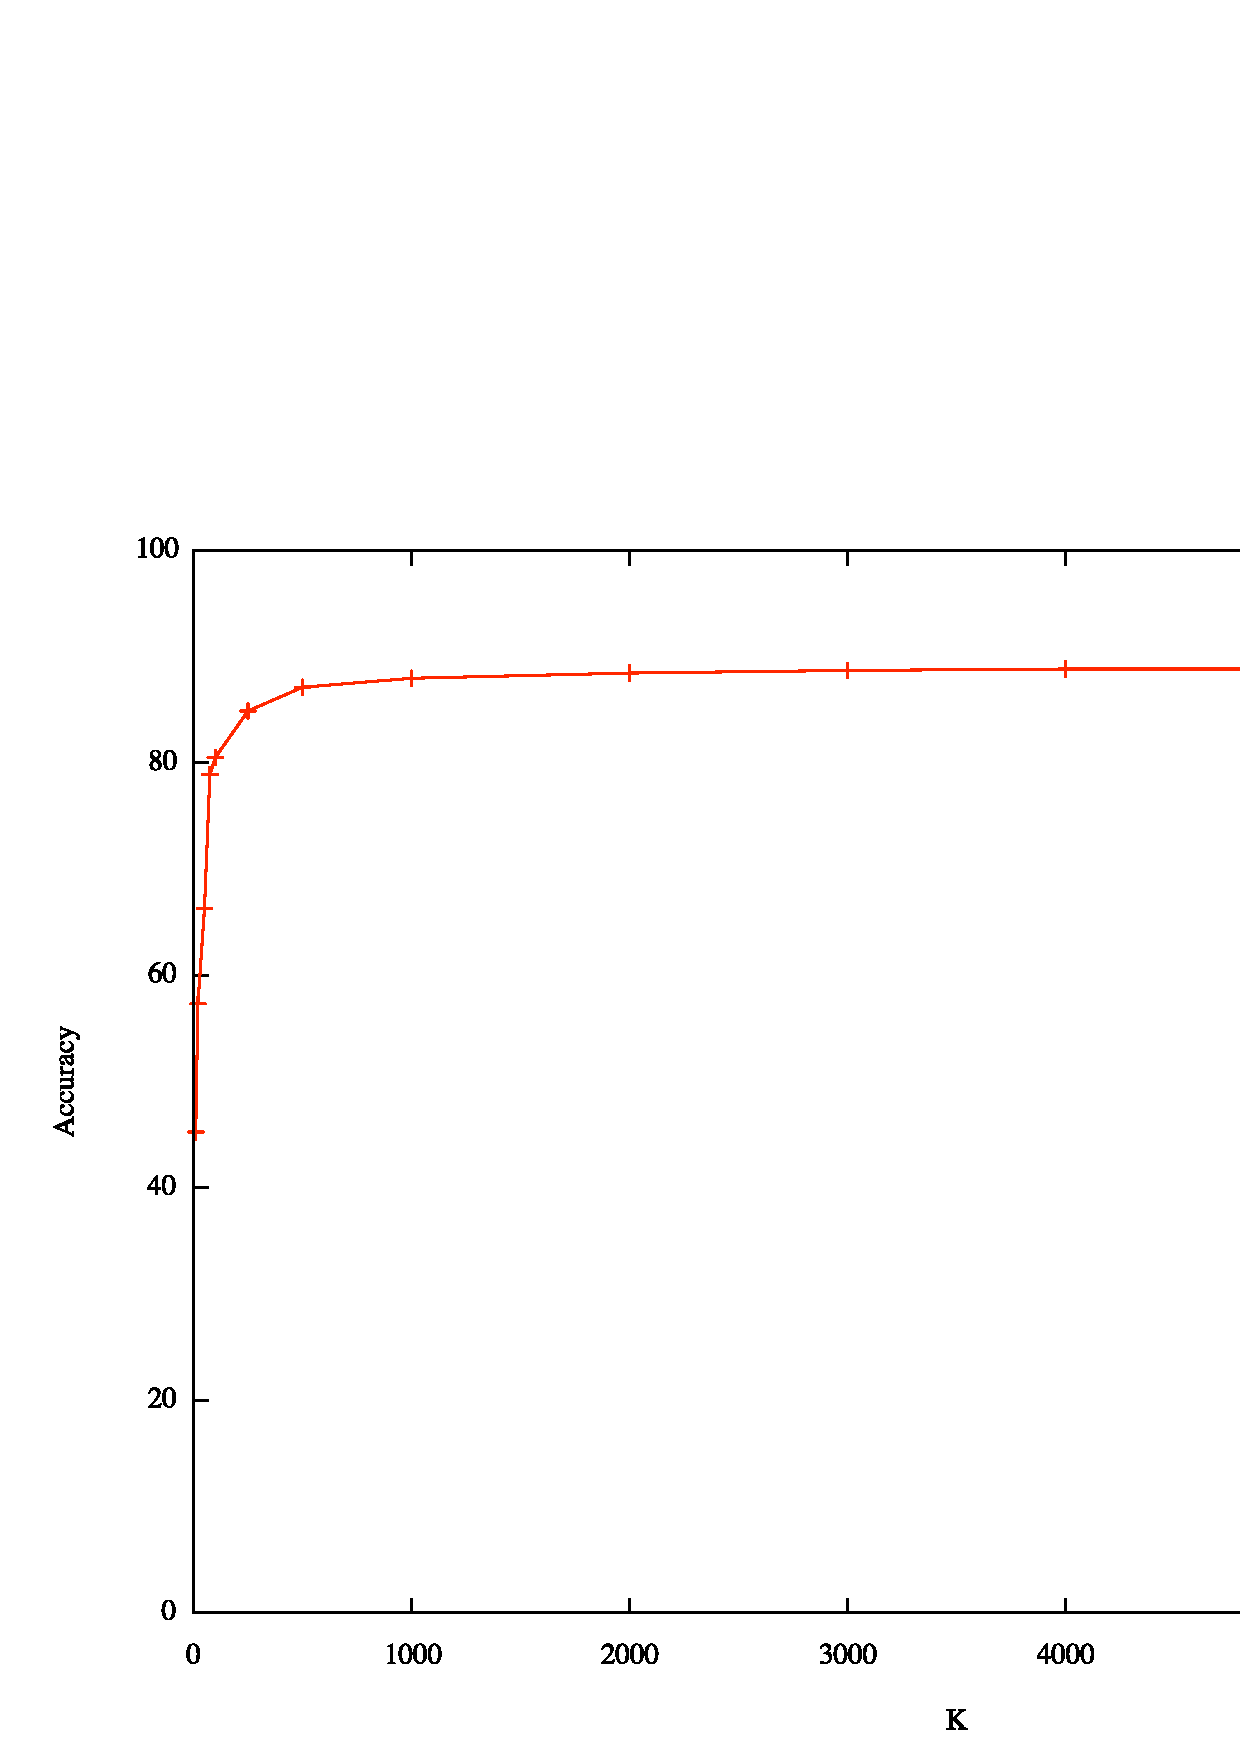
\includegraphics[totalheight=0.25\textheight]{DiffTrainSizes}
\caption{Learning curve of the average performance of our system, as a
  function of the number of training examples. This experiment is done
  with $K=3$ on the {\em TestWiki} test set.}
\label{fig:diff-train-size}
\end{figure}

%%% Local Variables: 
%%% mode: latex
%%% TeX-master: "jupiter"
%%% End: 
